\documentclass{article}
\usepackage{graphicx}
\setlength\parindent{0pt}
\usepackage{amsmath}
\usepackage{bm}

\begin{document}
	
	\section{Understanding word2vec}
	
	The key insight behind word2vec is that `a word is known by the company it keeps'. Concretely, suppose we have a `center' word $c$ and a contextual window surrounding $c$. We shall refer to words that lie in this contextual window as `outside words'. For example, in Figure 1 we see that the center word c is `banking'. Since the context window size is 2, the outside words are `turning', `into', `crises', and `as'.
	
	The goal of the skip-gram word2vec algorithm is to accurately learn the probability distribution $P(O|C)$. Given a specific word $o$ and a specific word $c$, we want to calculate $P(O=o|C=c)$, which is the probability of the word $o$ is an `outside' word for $c$, i.e., the probability that $o$ falls within the contextual windows of $c$. 
	
	\begin{figure}[h]
		\centering
		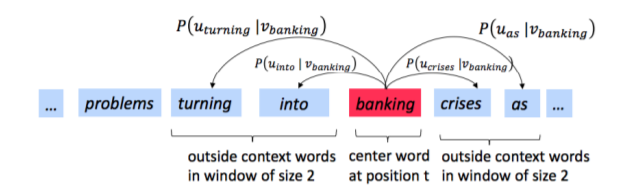
\includegraphics[width=0.7\linewidth]{skip-gram}
		\caption{The word2vec skip-gram prediction model with windows size 2}
		\label{fig:skip-gram}
	\end{figure}

	In word2vec, the conditional probability distribution is given by taking vector dot-products and applying the softmax function:
	
	\begin{equation}
		P(O=o|C=c) = \frac{exp(\bm{u}_o^\top \bm{v}_c)}{\Sigma_{w \in {Vocab}} exp(\bm{u}_w^\top)\bm{v}_c}	
		\label{eq:softmax}
	\end{equation}
	
	Here, $\bm{u}_o$ is the `outside' vector representing outside word $o$, and $v_c$ is the center `center' vector representing center word c. To contain these parameters, we have two matrices, $\bm{U}$ and $\bm{V}$. The columns of $U$ are all the `outside' vectors $u_w$. The columns of $\bm{V}$ are all the `center' vectors $v_w$. Both $\bm{U}$ and $\bm{V}$ contain a vector for every $w \in Vocabulary$.\footnote{Assume that every word in our vocabulary is matched to an integer number $k$. $\bm{u}_k$ is both the $k^{th}$ column of $\bm{U}$ and `outside' word vector for the word indexed by $k$. $\bm{v}_k$ is both the $k_{th}$ column of $\bm{V}$ and the `center' word vector for the word indexed by k. In order to simplify notation we shall interchangeably use $k$ to refer to the word and the index-of-the-word.}
	
	Recall that, for a single pair of words $c$ and $o$, the loss is given by:
	
	\begin{equation}
		\bm{J}_{naive-softmax}\bm{(v_c, o, U)} = -\log{P(O=o|C=c)}.
	\end{equation}
	
	Another way to view this loss is the cross-entropy\footnote{The Cross Entropy Loss between the true (discrete) probability distribution $p$ and another probability distribution $q$ is $-Sigma_{i} p_i \log{(q_i)}$.} between the true distribution $\bm{y}$ and the predicted distribution $\hat{\bm{y}}$. Here, both $\bm{y}$ and $\bm{\hat{y}}$ are the vectors with length equal to the number of words in the vocabulary. Furthermore, the $k^{th}$ entry in these vectors indicates the conditional probability of the $k^{th}$ word being an `outside word' for the given $c$. The true empirical distribution $\bm{y}$ is a one-hot vector with a 1 for the true outside word $o$, and 0 everywhere else. The predicted distribution $\hat{\bm{y}}$ is the probability distribution $P(O|C=c)$ given by our model in the equation \ref{eq:softmax}. 
	
	
	
\end{document}